\subsection{In-Depth Analysis of \syst}

\begin{table}[t]
    \centering
    \caption{\bf Detailed Ablation Studies on PAT (Qwen3-8B).}
    \vspace{-1em}
    \label{tbl:ablation_results_split}
    
    % --- Subtable 1: Cold Start ---
    \begin{subtable}[t]{0.88\columnwidth}
        \centering
        \caption{\bf{Ablation study on Cold Start stage. OSL represent Operator syntax Learning module in Section~\ref{subsec:cold_start}.}}
        \label{subtbl:cold_start}
        \vspace{-0.5em}
        \resizebox{0.99\linewidth}{!}{
        \begin{tabular}{|c||c|c|c|c|c|c|}
            \hline
            \multirow{2}{*}{\textbf{Method}} & \multicolumn{2}{c|}{\textbf{Synth-Spider}} & \multicolumn{2}{c|}{\textbf{Synth-Bird}} & \multicolumn{2}{c|}{\textbf{Parrot}} \\ \cline{2-7}
             & \textbf{Acc.} & \textbf{Comp.} & \textbf{Acc.} & \textbf{Comp.} & \textbf{Acc.} & \textbf{Comp.} \\
            \hline \hline
            % Row 1: Curriculum SFT
            Cold-Start & \textbf{60.66} & \textbf{91.63\%} & \textbf{45.27} & \textbf{81.39\%} & \textbf{36.22} & \textbf{92.16\%} \\
            % Row 2: w/o Operator Learning
            w/o OSL & {59.65} & {90.54\%} & {43.30} & {80.43\%} & {36.15} & {91.08\%} \\
            \hline
        \end{tabular}
        }
    \end{subtable}
    
    \vspace{0.5em}
    
    % --- Subtable 2: Multiturn RL ---
    \begin{subtable}[t]{0.93\columnwidth}
        \centering
        \caption{\bf{Ablation study on the reward of Multiturn RL stage.}}
        \label{subtbl:rl_stage}
        \vspace{-0.5em}
        \resizebox{0.99\linewidth}{!}{
        \begin{tabular}{|c||c|c|c|c|c|c|}
            \hline
            \multirow{2}{*}{\textbf{Method}} & \multicolumn{2}{c|}{\textbf{Synth-Spider}} & \multicolumn{2}{c|}{\textbf{Synth-Bird}} & \multicolumn{2}{c|}{\textbf{Parrot}} \\ \cline{2-7}
             & \textbf{Acc.} & \textbf{Comp.} & \textbf{Acc.} & \textbf{Comp.} & \textbf{Acc.} & \textbf{Comp.} \\
            \hline \hline
            % Row 1: V0-v1-v2 (Full sysem)
            \sys & \textbf{65.99} & \underline{97.46\%} & \textbf{53.39} & \underline{92.78\%} & \textbf{39.93} & \underline{98.46\%} \\
            % Row 2: v0-v1 (w/o R_llm)
            w/o $R_{\text{llm}}$ & \underline{64.54} & 96.96\% & \underline{51.67} & 92.31\% & \underline{39.12} & 94.21\% \\
            % Row 3: v0 (w/o R_llm, R_part)
            w/o $R_{\text{llm}}, R_{\text{part}}$ & 61.85 & \textbf{98.71\%} & 47.15 & \textbf{95.57\%} & 37.22 & \textbf{99.34\%} \\
            \hline
        \end{tabular}
        }
    \end{subtable}
    
  \vspace{-1em}
\end{table}


\noindent
\textbf{Exp-\expnum\label{exp:ablation_analysis}: Ablation studies on our policy learning method.}
We conduct ablation studies to verify the specific contributions of different components in our multi-stage policy learning method (Section~\ref{sec:agentic_training_framework}). The results are summarized in Table~\ref{tbl:ablation_results_split}.

% \textbf{Effectiveness of Cold-Start Curriculum.}
As illustrated in Table~\ref{subtbl:cold_start}, removing the Operator Learning (OL) phase leads to a consistent performance drop across all datasets. For instance, the accuracy on DP-Spider decreases from 60.11\% to 58.52\%.
This demonstrates that OL is essential for ``warming up" the model.
% \textbf{Necessity of Hybrid Reward in RL.}
Table~\ref{subtbl:rl_stage} investigates the impact of different reward components in the RL stage.
First, removing the LLM-as-Judge reward (w/o $R_{llm}$) leads to a clear drop in accuracy. This shows that $R_{llm}$ is key to checking the overall logic and preventing ``reward hacking''. For example, our logs showed that without this check, the model tried to cheat: it simply renamed columns to match the target schema to get partial rewards ($R_{partial}$), while skipping the actual data cleaning steps.
Second, when using only the outcome reward (w/o $R_{llm}, R_{partial}$), the Completion Rate grows, while the Accuracy drops a lot. 
This suggests that the model tends to become conservative. To avoid formatting penalties, it avoids the complex exploration and backtracking needed by our framework.

\begin{shaded}
\noindent \textbf{Finding \findingnum: Each module in our multi-stage strategy contributes to the final robust performance.}
\end{shaded}


\begin{figure}[t]
    \centering
    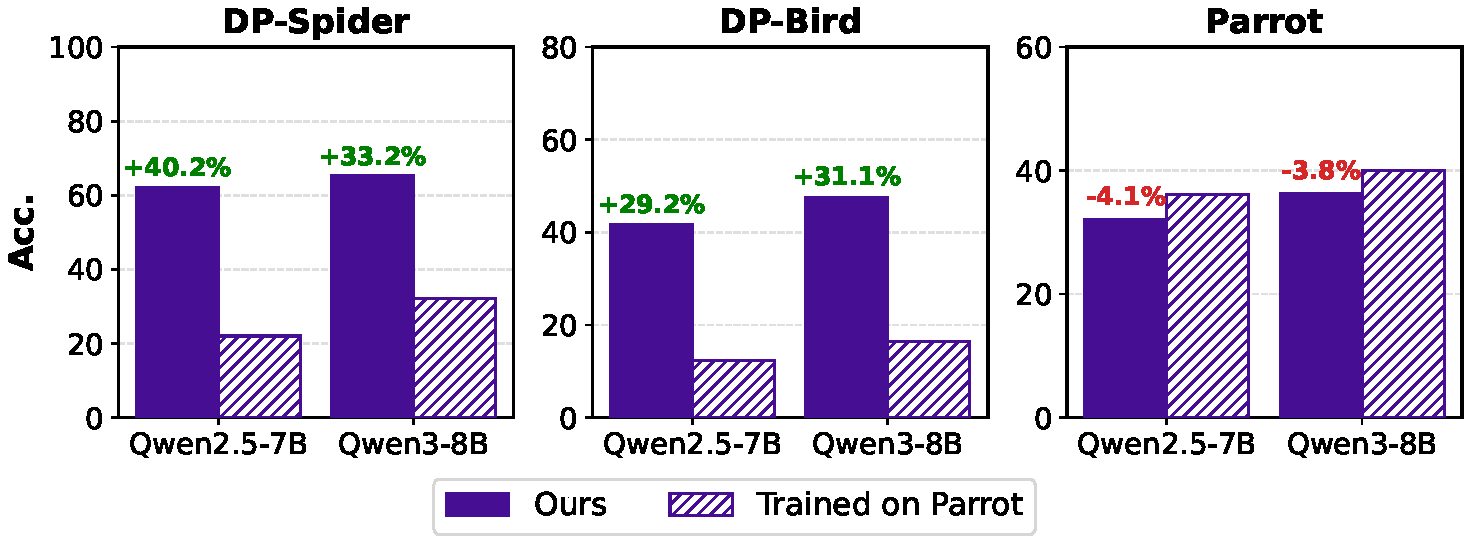
\includegraphics[width=0.99\columnwidth]{plots/plot/trained_on_parrot_accuracy.pdf}
    \vspace{-1em} 
    \caption{Accuracy trained on DP-Spider and Parrot.}
    \label{fig:trained_on_parrot_accuracy}
  \vspace{-0.5em}
\end{figure}
\begin{figure}[t]
    \centering
    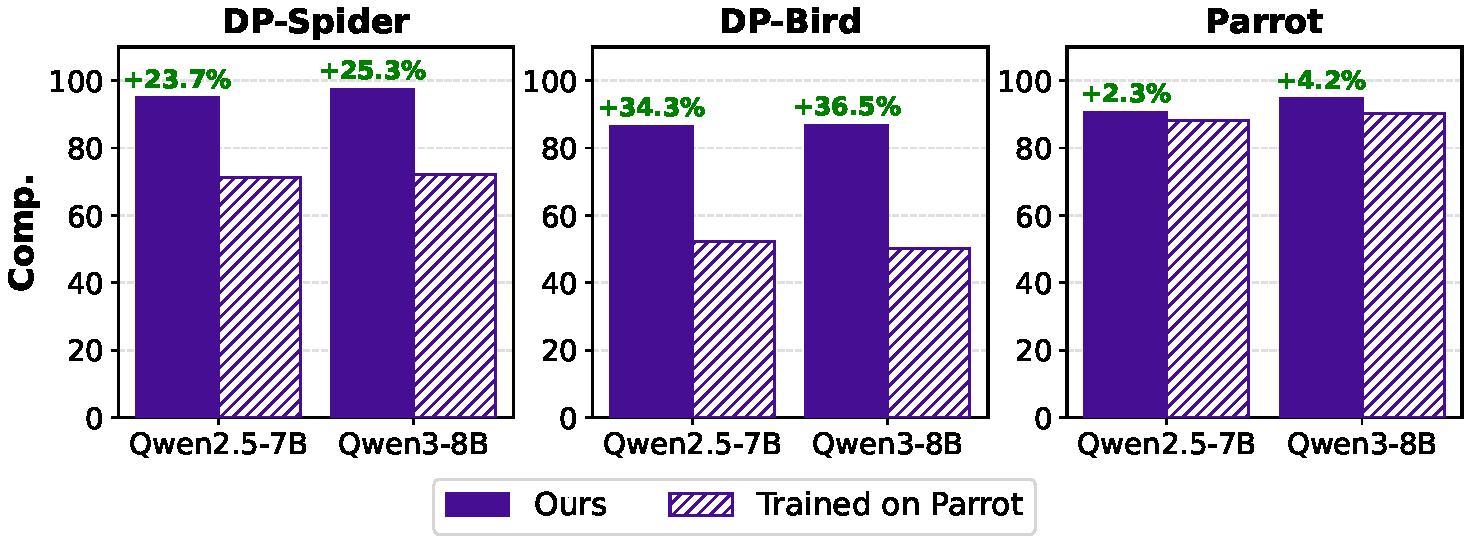
\includegraphics[width=0.99\columnwidth]{plots/plot/trained_on_parrot_complete_rate.pdf}
    \vspace{-1em} 
    \caption{Completion Rate trained on DP-Spider and Parrot.}
    \label{fig:trained_on_parrot_complete_rate}
  \vspace{-0.5em}
\end{figure}

\noindent
\textbf{Exp-\expnum\label{exp:trained_on_synthesized_or_public_data}: Comparison of \syst trained on our synthesized dataset and public dataset.}
To demonstrate the effectiveness of our scalable data synthesis method, we compare models trained on our synthesized data (DP-Spider) against those trained on the public dataset (Parrot). 
As illustrated in Figure~\ref{fig:trained_on_parrot_accuracy}, while training on Parrot yields a slight accuracy gain on its own test set, it causes a sharp drop on DP-Spider ($\sim$40\%) and DP-Bird ($\sim$30\%), indicating that the public dataset fails to equip the model with general reasoning skills. Furthermore, in Figure~\ref{fig:trained_on_parrot_complete_rate}, the Completion Rate decreases across all datasets when trained on Parrot. 
This is because models trained on our synthesized data better learn to perform global error correction, since errors are common for these challenging DP cases. 
In addition, we observe an emergent capability on complex tasks for models trained on our data: the model first explores using operators. When exceeding the turn limit without success, it switches to generate code with \texttt{ExeCodeeration} operator to complete the remaining operations in a single step. 
This confirms that our synthesized data, which covers diverse scenarios, is essential for building a robust agent capable of stable execution.

% To explain it, we find that training on our complex data enables the model to combine operators and code effectively: for hard tasks, the model first explores with operators, and if it exceeds the turn limit without success, it switches to code generation to finish the remaining operations in one step. This confirms that our synthesized data, which covers diverse scenarios, is essential for building a robust agent capable of stable execution.

\begin{shaded}
\noindent
\textbf{Finding \findingnum: Our synthesized data fosters stronger generalization capability compared with public dataset.}
\end{shaded}

\begin{figure}[t]
    \centering
    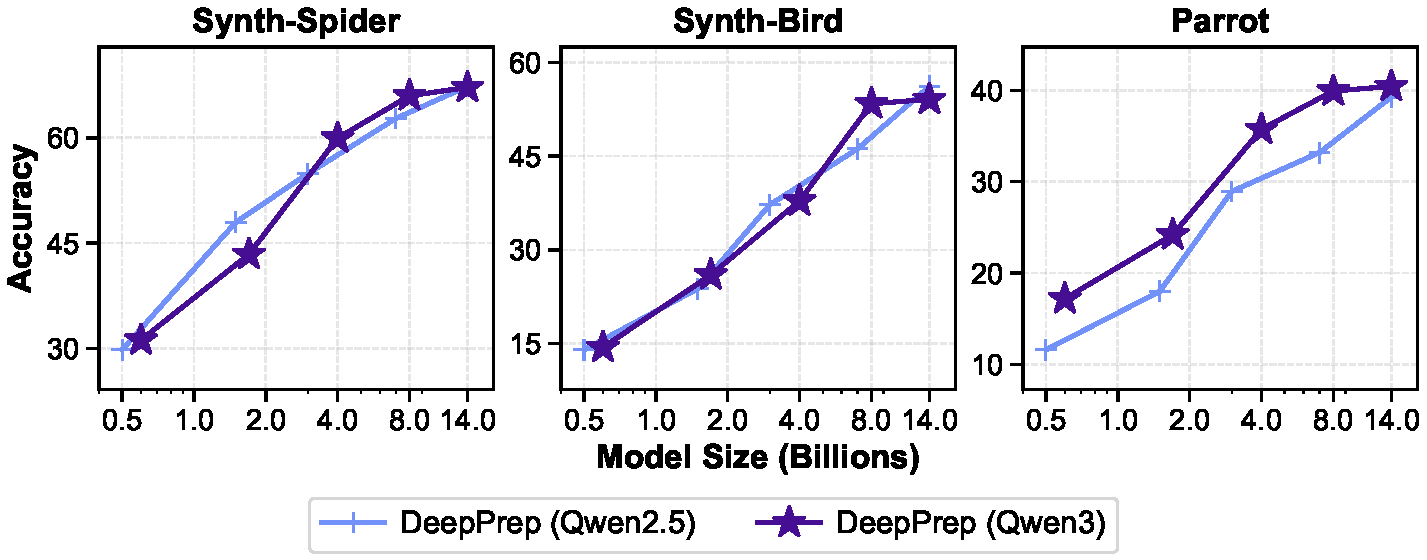
\includegraphics[width=1.01\columnwidth]{plots/plot/performance_scale_accuracy_only.pdf}
    \vspace{-1.5em} 
    \caption{Performance scales with larger model size.
    % \fmh{Results of Qwen2.5 are not updated (Use 2025 version).} 
    }
    \label{\labelprefix fig:performance_scale_accuracy_only}
    \vspace{-0.5em} 
  %\vspace{-1em}
\end{figure}

\noindent
\textbf{Exp-\expnum\label{exp:perfroamce_scale_on_varisou_model_size}: Can the performance of \syst scale with increasing model sizes?}
To answer this, we trained \syst using different LLM backbones (Qwen2.5 and Qwen3) ranging from 0.5B to 8B parameters. As shown in Figure~\ref{fig:performance_scale_with_larger_model_size}, both Accuracy and Completion Rate improve steadily as the model size increases. Specifically, on DP-Spider, scaling Qwen2.5 from 0.5B to 7B boosts Accuracy from 30.28\% to 62.35\%. Furthermore, we find that Qwen3 shows stronger generalization than Qwen2.5. For example, on the complex DP-Bird dataset, Qwen3-8B achieves 47.53\% accuracy, outperforming Qwen2.5-7B (41.58\%). This indicates that 
\syst can improve further as stronger open-source models are released.
% our training method is effective across different model generations, allowing \syst to improve further as stronger open-source models are released.

\begin{shaded}
\noindent
\textbf{Finding \findingnum: The performance of \syst scales consistently on stronger LLM backbones with larger model size.}
\end{shaded}